\begin{figure}
    % WARNING: DO NOT CHANGE MANUALLY, CHANGES WILL BE OVERWRITTEN
        \ifdefined\AAAINV\else
        \newcommand\A[2]{\mathbf{A}_{#2}^{#1}}
        \newcommand\B[2]{\mathbf{B}_{#2}^{#1}}
        \newcommand\AINV[2]{(\A{#1}{#2})^{-1}}
        \newcommand\BINV[2]{(\B{#1}{#2})^{-1}}
        \newcommand\AAA[1]{\mathbf{A}^{#1}}
        \newcommand\BBB[1]{\mathbf{B}^{#1}}
        \newcommand\AAAINV[1]{(\AAA{#1})^{-1}}
        \newcommand\BBBINV[1]{(\BBB{#1})^{-1}}
        \newcommand\R{\mathbf{R}}
        \newcommand\RINV{\mathbf{R}^{-1}}
        \newcommand\M{\mathbf{M}}
        \newcommand\El{\ell'}
        \newcommand\MINV{\mathbf{M}^{-1}}
        \newcommand\Min{m_{in}}
        \newcommand\Mout{m_{out}}
        \newcommand\XOR[1]{\mathbf{X}\left[#1\right]}
        \fi
        \ifdefined\aCipher\else
        \newcommand\aCipher{\texttt{Sparkle}}
        \newcommand\FigDef[2]{\caption{#2}\label{#1}}
        \newcommand\PathFig[1]{NON_EXISTANT_PATH/#1}
        \fi
    \FigDef{high-level}{The High-level structure of \aCipher{} with 4 steps.}
    \IfFileExists{\PathFig{Sparkle.pdf}}{
    \includegraphics{\PathFig{Sparkle.pdf}}
    }{
    \centering
    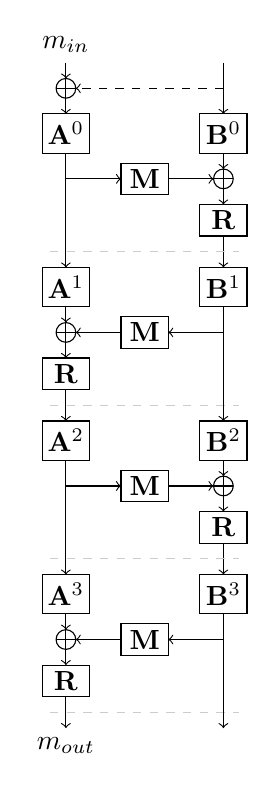
\begin{tikzpicture}[xscale=1.0,yscale=-1.0]
        \draw (0.0,0.0) node[anchor=south] {$\Min$};
        \draw[->] (0.0,0.0) -- (0.0,0.2);
        \draw (0.0,0.325) ellipse (0.125 and 0.125);
        \draw (0.0,0.2) -- (0.0,0.45);
        \draw (-0.125,0.325) -- (0.125,0.325);
        \draw (2.0,0.0) -- (2.0,0.325);
        \draw[->,dashed] (2.0,0.325) -- (0.125,0.325);
        \draw[->] (0.0,0.45) -- (0.0,0.65);
        \draw (-0.3,0.65) rectangle (0.3,1.15) node[pos=0.5] {$\AAA{0}$};
        \draw[->] (2.0,0.325) -- (2.0,0.65);
        \draw (1.7,0.65) rectangle (2.3,1.15) node[pos=0.5] {$\BBB{0}$};
        \draw (0.0,1.15) -- (0.0,1.475);
        \draw[->] (2.0,1.15) -- (2.0,1.35);
        \draw (2.0,1.475) ellipse (0.125 and 0.125);
        \draw (2.0,1.35) -- (2.0,1.6);
        \draw (1.875,1.475) -- (2.125,1.475);
        \draw[->] (0.0,1.475) -- (0.7,1.475);
        \draw (0.7,1.275) rectangle (1.3,1.675) node[pos=0.5] {$\M$};
        \draw[->] (1.3,1.475) -- (1.875,1.475);
        \draw[->] (2.0,1.6) -- (2.0,1.8);
        \draw (1.7,1.8) rectangle (2.3,2.2) node[pos=0.5] {$\R$};
        \draw (0.0,1.475) -- (0.0,2.4);
        \draw (2.0,2.2) -- (2.0,2.4);
        \draw[dashed,gray!40] (-0.2,2.4) -- (2.2,2.4);
        \draw[->] (0.0,2.4) -- (0.0,2.6);
        \draw (-0.3,2.6) rectangle (0.3,3.1) node[pos=0.5] {$\AAA{1}$};
        \draw[->] (2.0,2.4) -- (2.0,2.6);
        \draw (1.7,2.6) rectangle (2.3,3.1) node[pos=0.5] {$\BBB{1}$};
        \draw[->] (0.0,3.1) -- (0.0,3.3);
        \draw (0.0,3.425) ellipse (0.125 and 0.125);
        \draw (0.0,3.3) -- (0.0,3.55);
        \draw (-0.125,3.425) -- (0.125,3.425);
        \draw (2.0,3.1) -- (2.0,3.425);
        \draw[->] (2.0,3.425) -- (1.3,3.425);
        \draw (0.7,3.225) rectangle (1.3,3.625) node[pos=0.5] {$\M$};
        \draw[->] (0.7,3.425) -- (0.125,3.425);
        \draw[->] (0.0,3.55) -- (0.0,3.75);
        \draw (-0.3,3.75) rectangle (0.3,4.15) node[pos=0.5] {$\R$};
        \draw (0.0,4.15) -- (0.0,4.35);
        \draw (2.0,3.425) -- (2.0,4.35);
        \draw[dashed,gray!40] (-0.2,4.35) -- (2.2,4.35);
        \draw[->] (0.0,4.35) -- (0.0,4.55);
        \draw (-0.3,4.55) rectangle (0.3,5.05) node[pos=0.5] {$\AAA{2}$};
        \draw[->] (2.0,4.35) -- (2.0,4.55);
        \draw (1.7,4.55) rectangle (2.3,5.05) node[pos=0.5] {$\BBB{2}$};
        \draw (0.0,5.05) -- (0.0,5.375);
        \draw[->] (2.0,5.05) -- (2.0,5.25);
        \draw (2.0,5.375) ellipse (0.125 and 0.125);
        \draw (2.0,5.25) -- (2.0,5.5);
        \draw (1.875,5.375) -- (2.125,5.375);
        \draw[->] (0.0,5.375) -- (0.7,5.375);
        \draw (0.7,5.175) rectangle (1.3,5.575) node[pos=0.5] {$\M$};
        \draw[->] (1.3,5.375) -- (1.875,5.375);
        \draw[->] (2.0,5.5) -- (2.0,5.7);
        \draw (1.7,5.7) rectangle (2.3,6.1) node[pos=0.5] {$\R$};
        \draw (0.0,5.375) -- (0.0,6.3);
        \draw (2.0,6.1) -- (2.0,6.3);
        \draw[dashed,gray!40] (-0.2,6.3) -- (2.2,6.3);
        \draw[->] (0.0,6.3) -- (0.0,6.5);
        \draw (-0.3,6.5) rectangle (0.3,7.0) node[pos=0.5] {$\AAA{3}$};
        \draw[->] (2.0,6.3) -- (2.0,6.5);
        \draw (1.7,6.5) rectangle (2.3,7.0) node[pos=0.5] {$\BBB{3}$};
        \draw[->] (0.0,7.0) -- (0.0,7.2);
        \draw (0.0,7.325) ellipse (0.125 and 0.125);
        \draw (0.0,7.2) -- (0.0,7.45);
        \draw (-0.125,7.325) -- (0.125,7.325);
        \draw (2.0,7.0) -- (2.0,7.325);
        \draw[->] (2.0,7.325) -- (1.3,7.325);
        \draw (0.7,7.125) rectangle (1.3,7.525) node[pos=0.5] {$\M$};
        \draw[->] (0.7,7.325) -- (0.125,7.325);
        \draw[->] (0.0,7.45) -- (0.0,7.65);
        \draw (-0.3,7.65) rectangle (0.3,8.05) node[pos=0.5] {$\R$};
        \draw (0.0,8.05) -- (0.0,8.25);
        \draw (2.0,7.325) -- (2.0,8.25);
        \draw[dashed,gray!40] (-0.2,8.25) -- (2.2,8.25);
        \draw[->] (0.0,8.25) -- (0.0,8.45);
        \draw[->] (2.0,8.25) -- (2.0,8.45);
        \draw (0.0,8.45) node[anchor=north] {$\Mout$};
    \end{tikzpicture}
    }
\end{figure}
